\section{Introduction}

\begin{frame}{The Swarm at the Edge of the Cloud}
  \pause

  \begin{columns}
    \column{0.5\textwidth}
    \begin{figure}
      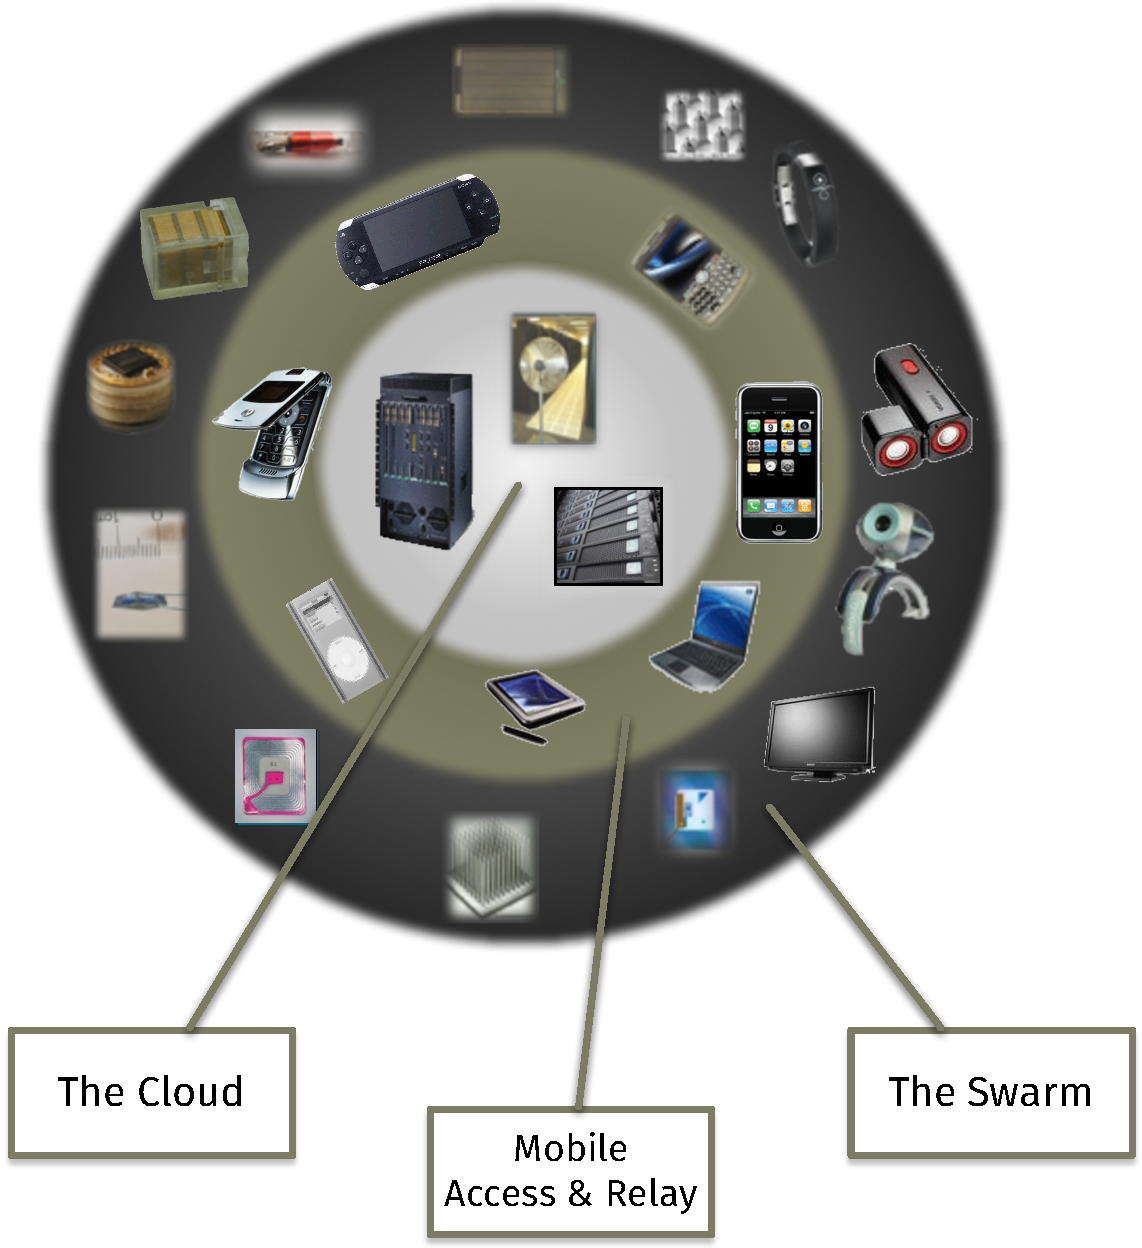
\includegraphics[width=\textwidth]{figures/swarm_jan.pdf}
      \caption{J.\,Rabaey, ASPDAC'08}
    \end{figure}

    \pause

    \column{0.5\textwidth}
    Swarm, or
    \begin{itemize}
    \item Internet of Things (IoT)
    \item Internet of Everything (IoE)
    \item Industry 4.0
    \item The Industrial Internet
    \item TSensors (Trillion Sensors)
    \item Machine to Machine (M2M)
    \item Smarter Planet
    \end{itemize}
  \end{columns}
\end{frame}

\begin{frame}{SwarmLab and TerraSwarm}

\end{frame}

\begin{frame}[fragile, plain]
  \begin{figure}
    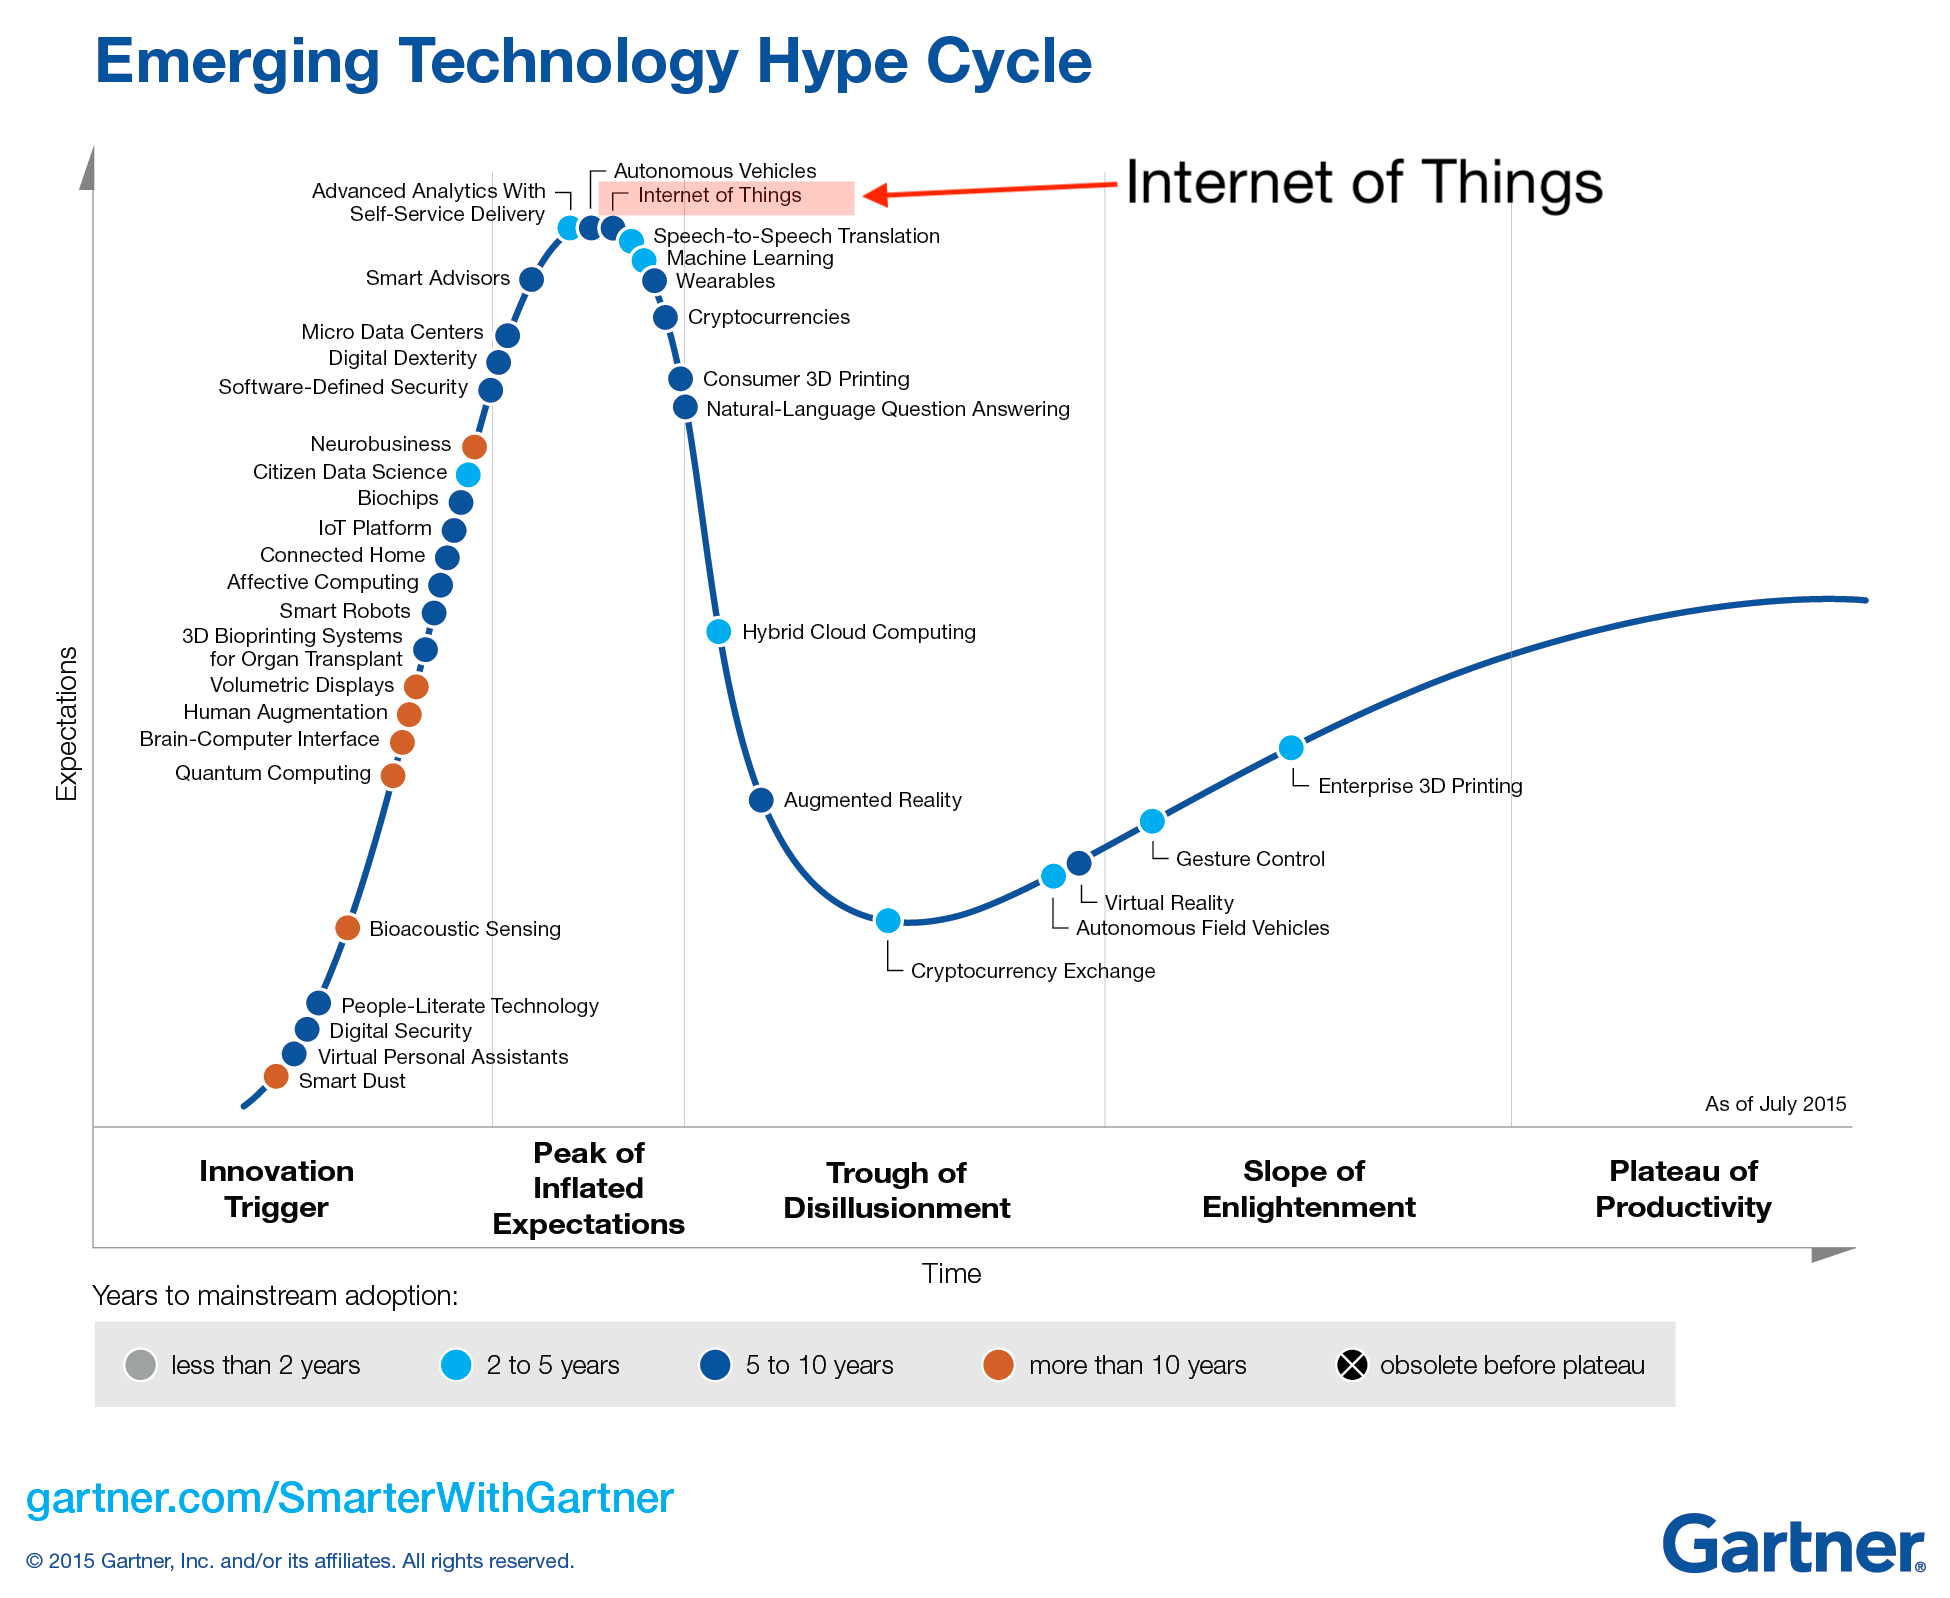
\includegraphics[width=\textwidth]{figures/hype.png}
  \end{figure}
\end{frame}

\begin{frame}{``Smart Things'' Formula}

  \begin{itemize}
  \item<1-> \textbf<1>{Thing}
  \item<2-> \textbf<2>{Thing + MCU (micro-controller)}
  \item<3-> \textbf<3>{Thing + MCU + Sensor/Actuator}
  \item<4-> \textbf<4>{Thing + MCU + Sensor/Actuator + Radio $\Rightarrow$ Connected}
  \item<5-> \textbf<5>{Thing + MCU + Sensor/Actuator + Radio + Gateway $\Rightarrow$ Internet}
  \item<5-> \textbf<6>{Thing + MCU + Sensor/Actuator + Radio + Gateway + Machine Learning}
  \end{itemize}

\end{frame}

\begin{frame}{Cloud Centric}
  \begin{columns}
    \column{0.5\textwidth}
    \begin{figure}
      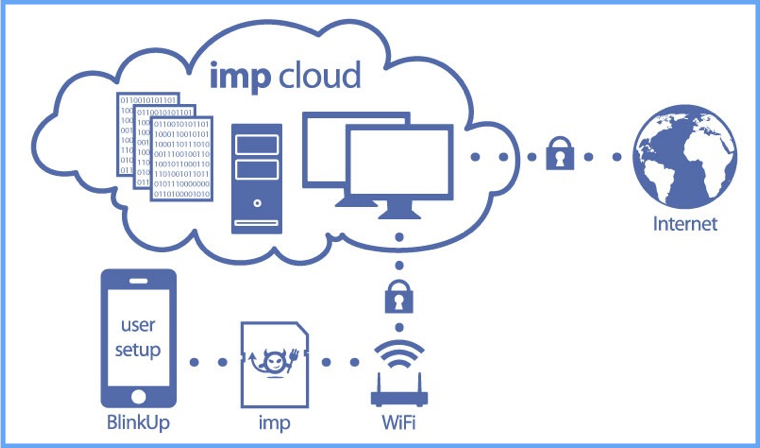
\includegraphics[width=\textwidth]{figures/cloud1.png}
      \captionsetup{labelformat=empty}
      \caption{Electric Imp: http://www.limetrace.co.uk/electric-imp-platform}
    \end{figure}

    \column{0.5\textwidth}
    \begin{figure}
      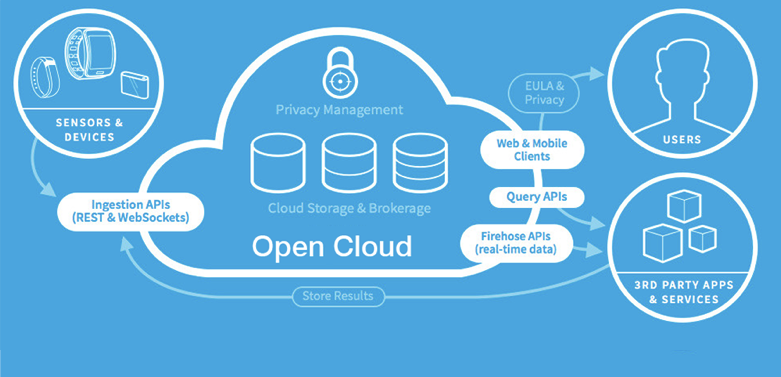
\includegraphics[width=\textwidth]{figures/cloud2.png}
      \captionsetup{labelformat=empty}
      \caption{Samsung SAMI: https://developer.samsungsami.io/sami/sami-documentation/}
    \end{figure}

    \begin{figure}
      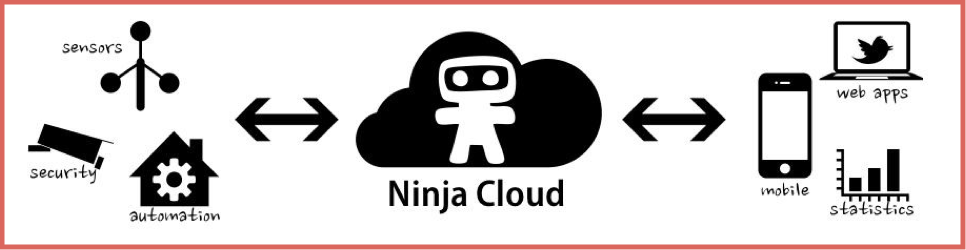
\includegraphics[width=\textwidth]{figures/cloud3.png}
      \captionsetup{labelformat=empty}
      \caption{Ninja Sphere: http://lucept.files.wordpress.com/2012/06/ninja-blocks-capture.jpg}
    \end{figure}
\end{columns}
\end{frame}

\begin{frame}{The Cloud is Not Enough}
  \begin{figure}
    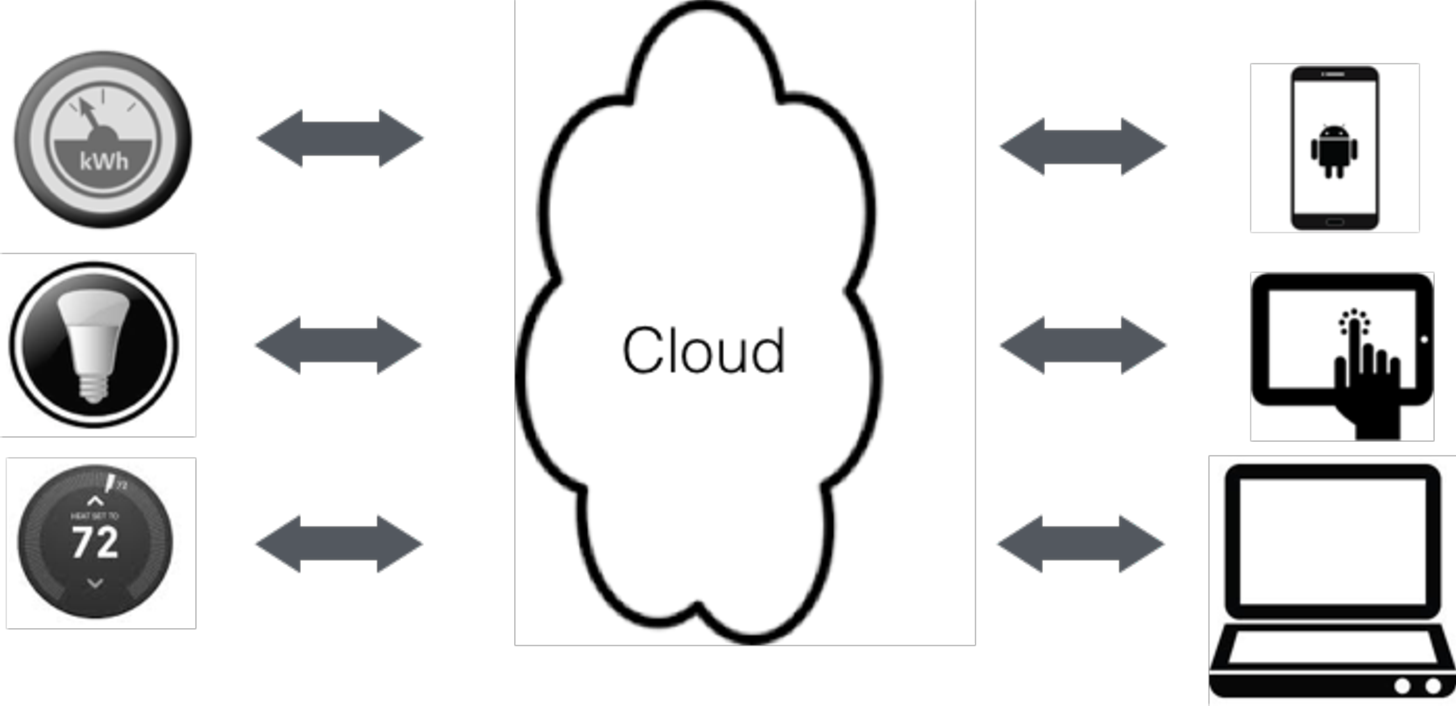
\includegraphics[width=0.6\textwidth]{figures/cloud-view.pdf}
  \end{figure}
  \vspace{-3em}
  \pause
  \begin{figure}
    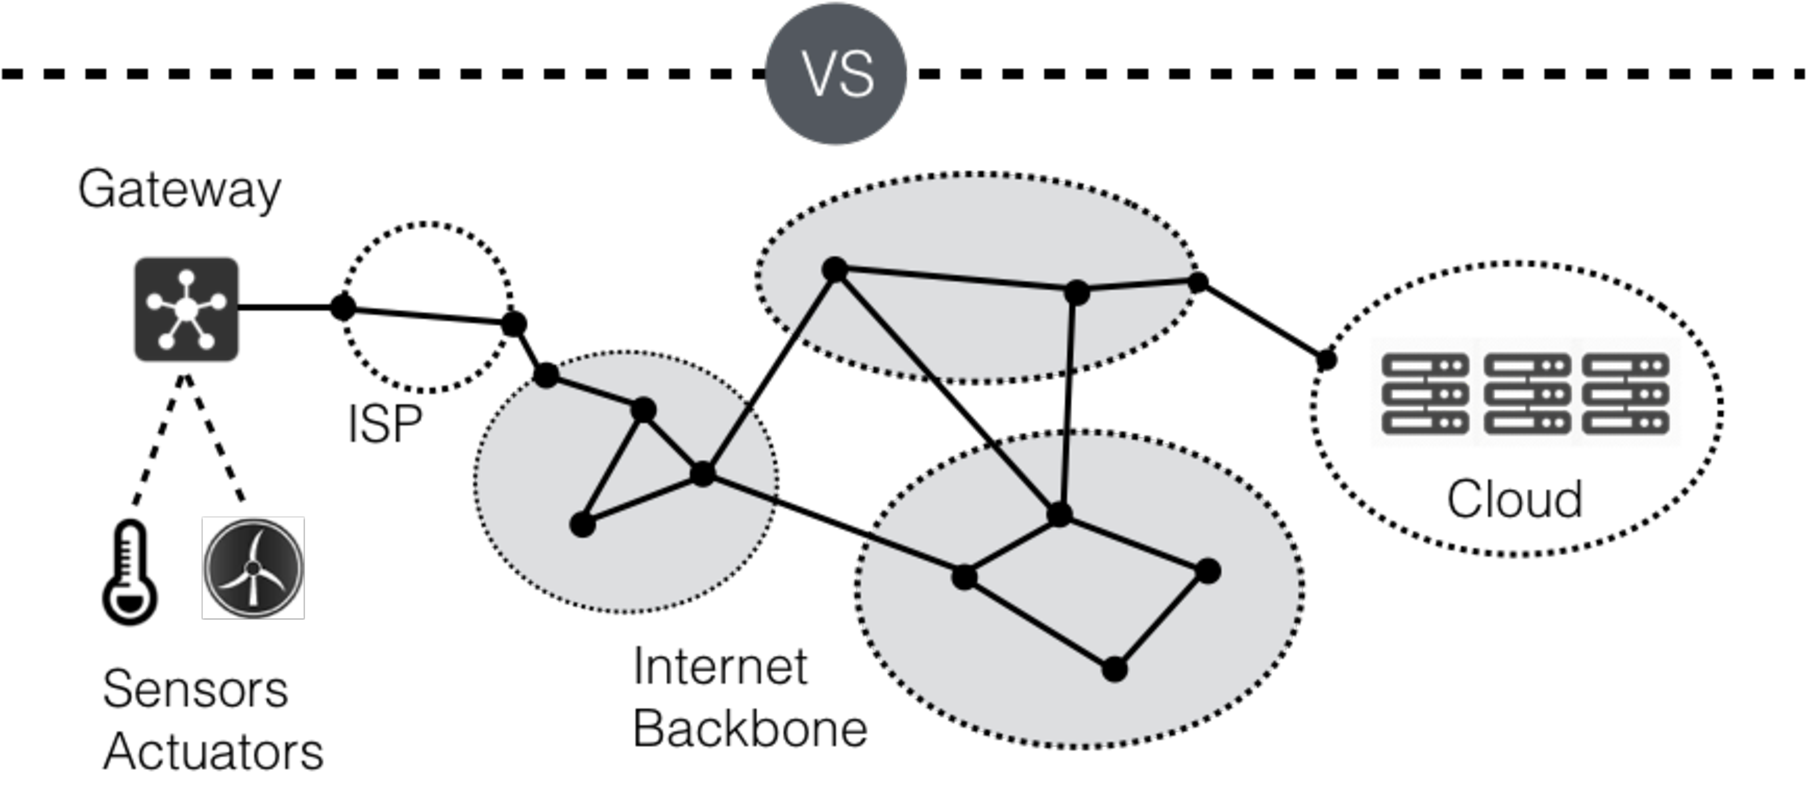
\includegraphics[width=0.7\textwidth]{figures/cloud-reality.pdf}
  \end{figure}
\end{frame}

\begin{frame}{What is Fundamentally Different?}

  \begin{table}
    \centering
    \begin{tabular}{c c c}
      \toprule
      & Web/IT & Swarm/IoT \\
      \midrule
      Privacy \& Security & Open for access & Personal sensitive data \\
      Scalability & Power law & Billion devices \& updates \\
      Interaction Model & Human & Machine \\
      Latency & Variable & Deterministic  \\
      Bandwidth & Downstream & Upstream   \\
      Availability (QoS) & No guarantee & Requirement  \\
      Durability Management & Cloud controls & Users control \\
      \bottomrule
    \end{tabular}
  \end{table}

\end{frame}

\begin{frame}{Bandwidth}
  \begin{figure}
    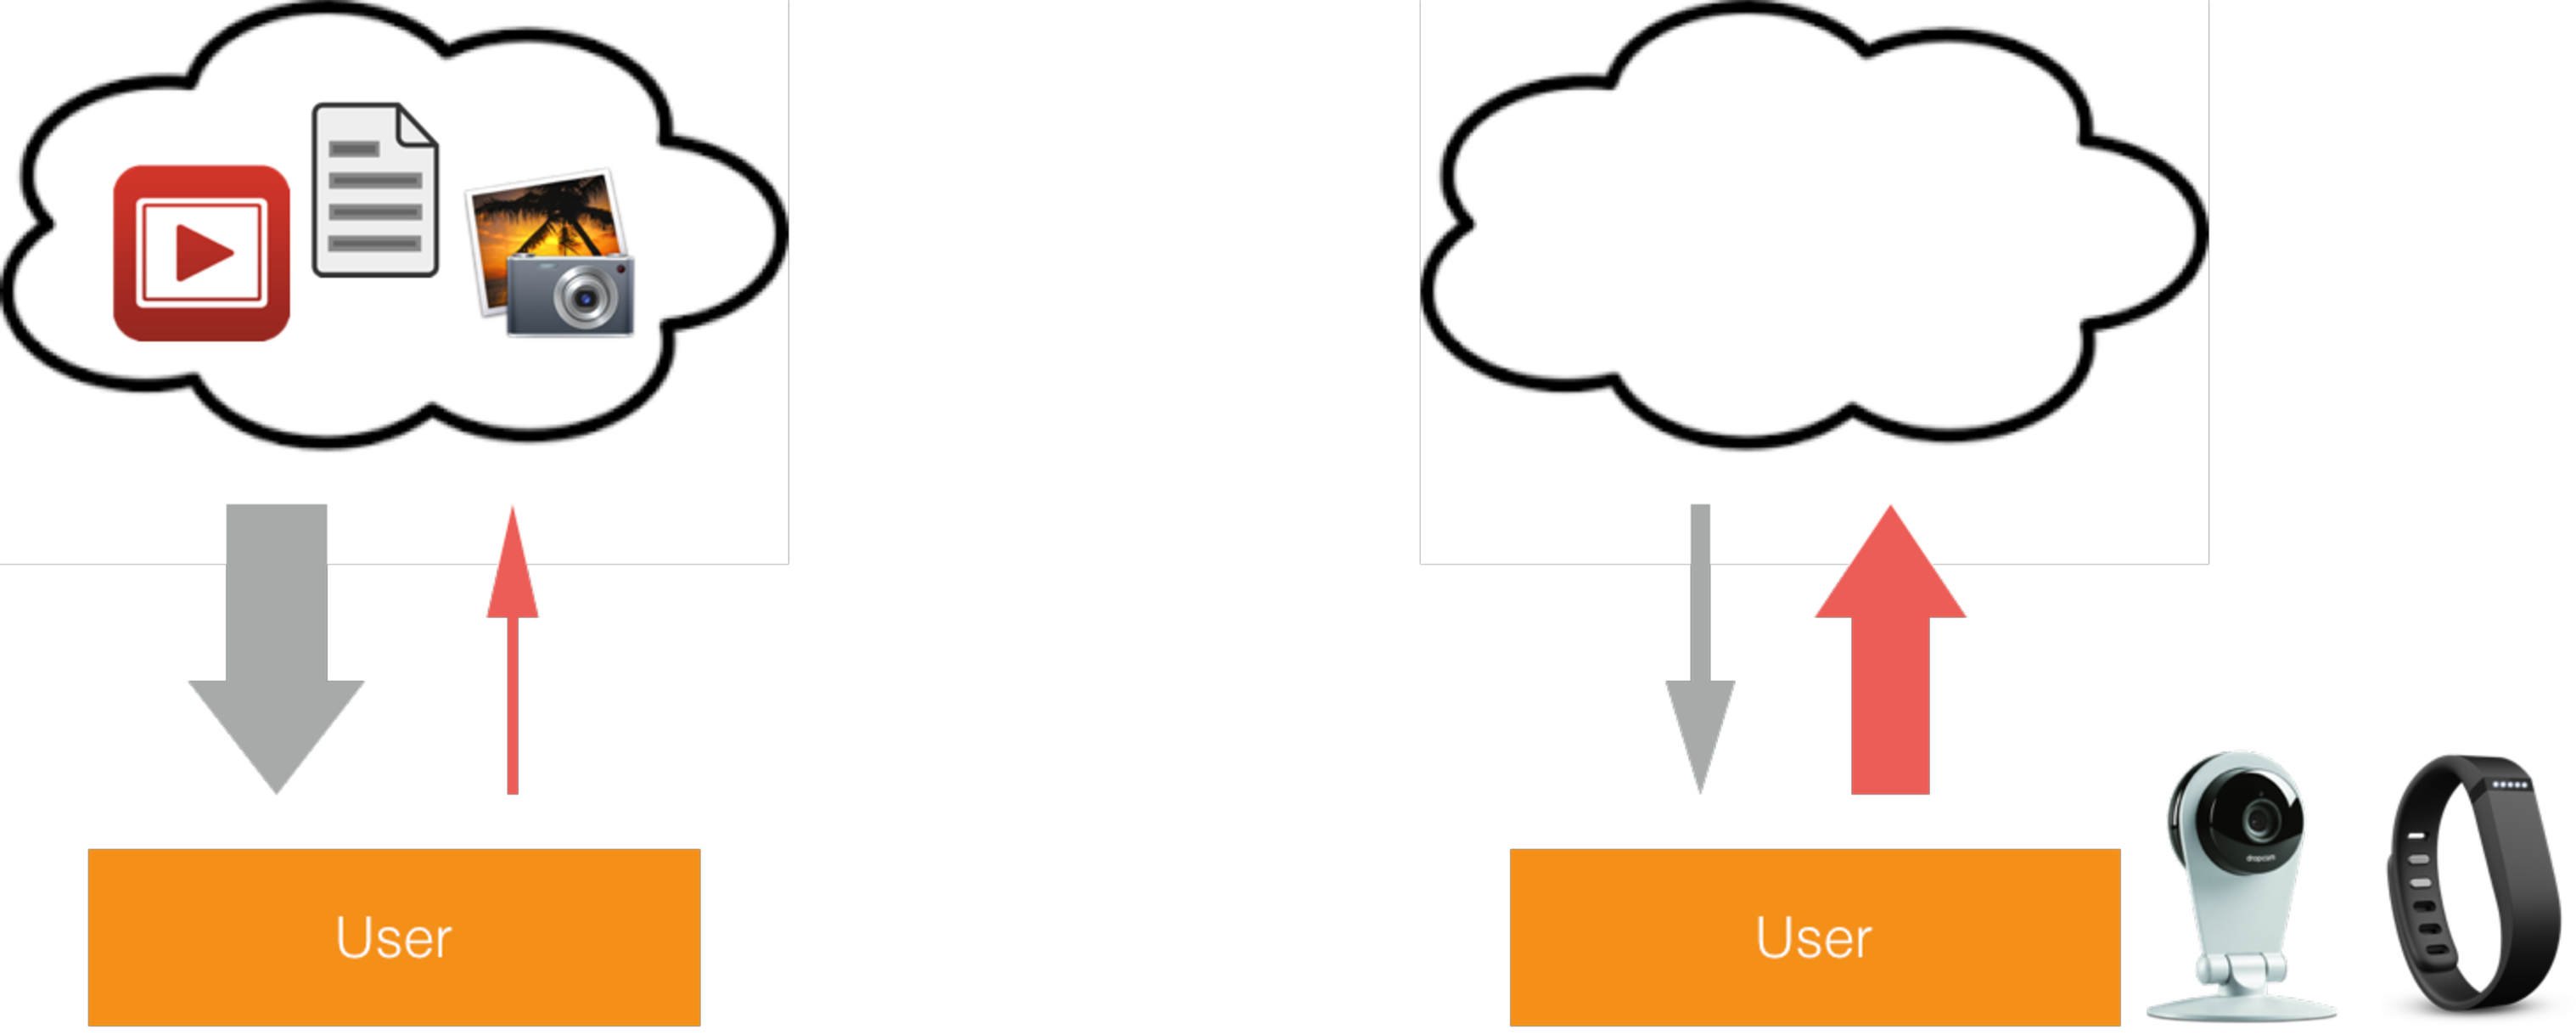
\includegraphics[width=\textwidth]{figures/upstream-downstream.pdf}
  \end{figure}
\end{frame}

\begin{frame}{Fog/Cloudlet/Swarmbox \& New Infrastructure}
  \begin{columns}
    \column{0.5\textwidth}
    \begin{figure}
      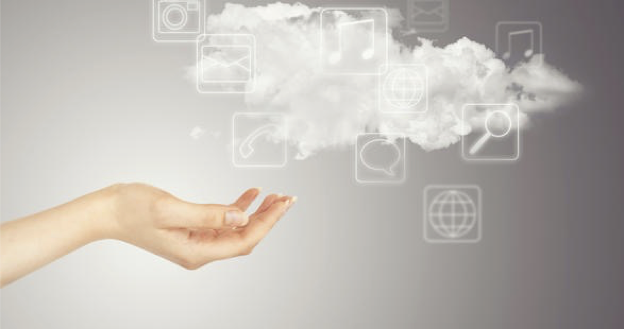
\includegraphics[width=0.8\textwidth]{figures/fog.png}
      \captionsetup{labelformat=empty}
      \caption{Cisco Fog Computing}
    \end{figure}
    \pause
    \column{0.5\textwidth}
    \begin{figure}
      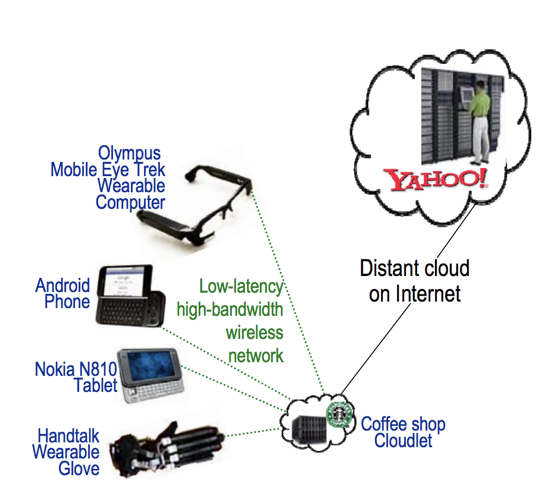
\includegraphics[width=0.8\textwidth]{figures/cloudlet.png}
      \captionsetup{labelformat=empty}
      \caption{CMU Cloudlet}
    \end{figure}
  \end{columns}
  \pause
  \begin{figure}
    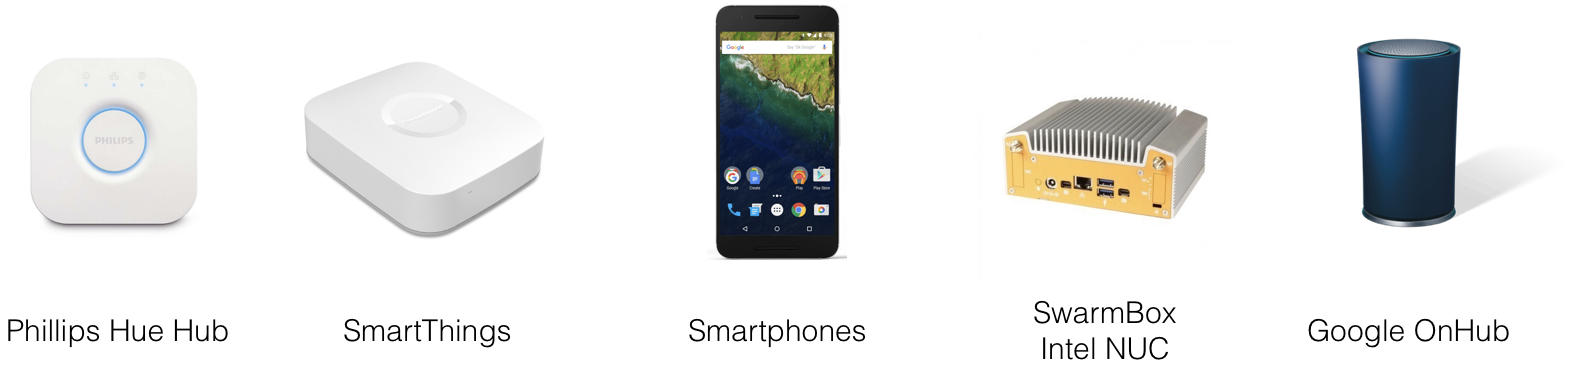
\includegraphics[width=0.8\textwidth]{figures/gateways.png}
    \captionsetup{labelformat=empty}
    \caption{Many Gateways}
  \end{figure}
\end{frame}

\begin{frame}{Adaptation}
  Challenges:
  \begin{itemize}
  \item Scarce and Limited WAN Bandwidth
  \item Heterogeneous Hardware/Computing
  \end{itemize}
\end{frame}

%%% Local Variables:
%%% mode: latex
%%% TeX-engine: xetex
%%% TeX-master: "talk"
%%% End:
